\section{Introduction}\label{sec:introduction}
The analysis of complex networks has become very important in recent times. Complex networks, especially social networks, are analyzed within the scope of data mining and valuable information is extracted. The valuable information obtained provides critical benefits in a wide range of areas. Community detection has an important place in the tools used to analyze such complex networks~\cite{ref:Fort}. If we come to the question of what communities are, there is no single definite definition yet. The general provision is that the communities are more tightly bound within themselves than they are in relation to the rest of the network. Members in communities are often members of more than one community. Detecting these communities brings various benefits to many areas. For advertising companies, for example, communities are important because there is a relationship that connects each community within itself. When this relationship is known, it is possible to make inferences through the common points of the people and to carry out highly efficient and targeted marketing~\cite{ref:Lancichinetti}. Available algorithms for discovering communities can often identify flat communities that do not intersect. A small number of algorithms have been included in the literature to detect intersecting communities. Almost all of these algorithms are built on the serial programming paradigm and are not preferred because they fail in large networks or because the runtime is too long ~\cite{ref:PhysRevE}. The main reason behind this situation is the fact that the dependencies between the communities are excessive and the clustering process is a time consuming process. Therefore, overlapping community detection is a computationally expensive and costly operation. On the other side, one of the most fundamental characteristics of social and biological networks is that the communities in the network are in a state of intersecting, that is, overlapping communities  ~\cite{ref:Gold}. Overlapping communities have more applications in the real world. Clique Percolation ~\cite{ref:Palla} and Link Clustering ~\cite{ref:LinkCls} methods are powerful methods proposed in this research domain. Unfortunately, even these methods are inadequate for real world applications involving millions of connections and are not scalable ~\cite{ref:Matrix}. 
In this work we try to solve the problem of discovering communities in large networks where data dependencies are much and overlapping communities are the majority. We need a system that can find both quality communities and work as fast as lightning.
There are some difficulties in detecting overlapping communities in large networks. First of all, data dependency poses a serious problem in parallel development. Since the networks we use are very large, we do not have the luxury of replicating the data. We need to partition the data. How to partition the data is a problem in itself. Both the communication should be kept at minimum level and the loads of the machines should be balanced. Our second problem is how to manage the communication process after partitioning the data to the machines. Data dependencies have negative effects on communication. At this point, it is of crucial importance to decide how to receive and send data. The third difficulty we are facing is the merging of communities that share common elements into a single community. Merge operation is performed according to a specified threshold value. Remember overlapping communities have common elements. If two communities contain a large number of common elements, why not sum them up in one community. Merge brings some problems with it. Comparing all communities among themselves will be quite time consuming and will undermine total speedup.
We tried to overcome the three main difficulties that we mentioned in the previous paragraph in various ways. First, we implemented different algorithms in the partitioning of the data to machines. We have written an algorithm that works like breadth first search logic, which provides both fast working and locality. To increase the success of this algorithm we partition the data to machines so that the total degree is equal. In addition to degree based BFS partitioning, we performed tests using Metis partitioning and random partitioning. The method used in partitioning directly affects communication. In order to complete the communication as soon as possible, we aim to make the communication processes as batch queries. In this direction we have defined 3 different communication approaches. In the first approach, we bring directly the adjacency information of the node that we need to know. This is done collectively in one go. Communication is carried out as batch queries after all the machines find out the boundary nodes. In the second approach, instead of bringing all the neighbors of a node, we are querying whether there is a connection between the boundary nodes that we need for neighborhood information. In our third approach, we combined the previous two approaches and developed a hybrid approach. That is, we look at how many neighbors does the boundary node has. If this node's neighbor number is less than all the connection information we want to know about that node, we choose the first method, the approach of bringing the neighbors directly. Otherwise we apply the second method. These queries are also done as batch requests like other queries. In the process of merging communities, our main problem is that there are so many communities and that it is difficult to compare all communities. As a matter of fact, it is not very logical to compare all communities with each other. Because the communities which have not common members are known at the beginning, there is no need to compare them with each other in the next stage. In this direction, we have developed a graph based merge algorithm that works by using inverted index mechanism. This merging technique improves the overall performance significantly.
In this direction, we have carried out research to create a fast-running and scalable parallel overlapping community detection system. As a result, we propose the system named Parocod. The Parocod is actually a system that runs the Demon ~\cite{ref:Demon} algorithm and the PCJ ~\cite{ref:Pcj} library in parallel. There are several reasons why we choose the PCJ library and Demon algorithm. First of all, the PCJ Library has emerged recently and has performed very well in terms of performance. In addition, PCJ provides a lot of convenience to the researcher during the coding phase and benefits from all the benefits of Java, a high-level programming language. PCJ adopts partitioned global address space approach and hides details of thread programming. The PCJ provides researcher to quickly develop distributed applications by focusing on the algorithm without drowning in details of the code. As overlapping community detection algorithm we prefer to use Demon algorithm. The Demon algorithm is the first choice because it works fast and gives good quality results and is very effective for parallel operation.
The Parocod consists of several stages. Partitioning is done in the first stage. The data is never replicated in another machine. The information of a node is stored in only one machine. Machines communicate with each other for nodes that are not in their own memory. Communication is carried out in the second phase, and the data that every machine needs is taken and given. In the third stage, each machine runs its own Demon algorithm and finds local communities, and according to the set threshold, if the communities contain certain members in common, the number of communities is reduced. In the fourth and last stage, machines send out the communities they found to the other machines to carry out a global merging process. We made various contributions and improvements at various stages in this process. We share detailed results in the experiment section. 
In this study, we aim to contribute the following:
\begin{itemize}
 \item A fast scalable parallel algorithm based on PCJ library for overlapping community detection over huge graphs .
 \item Three types of communication schemes; third one is degree oriented communication scheme. It is the hybrid of other two schemes. 
\item A merging technique relying on inverted index mechanism to speed up merging part.
 \item An extensive experimental evaluation of Paracod on real-world synthetic datasets, with respect to running time performance.
 \end{itemize}
The rest of the paper is organized as follows: in Section 2 we present related works in parallel overlapping community discovery literature. Section 3 is dedicated to the problem representation and definition. In Section 4, the Parocod is explained in detail. Section 5 describes the DEMON algorithm. Our experiments are presented in Section 6, and finally Section 7 concludes the paper.

This is a reference to a Section~\ref{sec:related}.

This is a reference to a Figure~\ref{fig:bugra1}.

This is a reference to a Table~\ref{tbl:data}.



\begin{figure*}[t]
\centering
\begin{minipage}{0.48\linewidth}
  \centering
  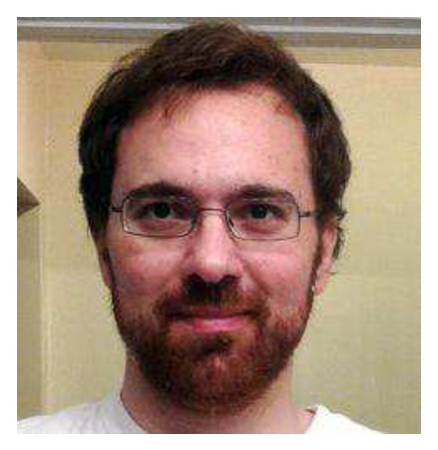
\includegraphics[width=0.5\linewidth]{figures/bugra.eps}
  \caption{Caption goes here}\label{fig:bugra1}
\end{minipage}
\vspace{0.01\linewidth}
\begin{minipage}{0.48\linewidth}
  \centering
  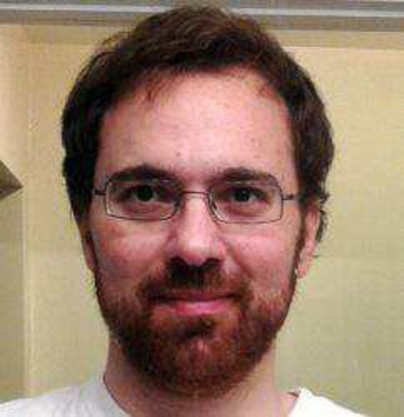
\includegraphics[width=0.5\linewidth]{figures/bugra.pdf}
  \caption{Caption goes here}\label{fig:bugra2}  
\end{minipage}
\end{figure*}


\begin{table*}[t]
\centering
\begin{tabular}{|l||c|c|c|}\hline 
\emph{props.}$\backslash$\emph{names} 
              & seqNo    & RIC     & Date         \\\hline
types         & long     & string  & string       \\\hline
sizes         & $0.08$   & $0.07$  & $0.15$       \\\hline
best alg.     & seq      & zlib    & sameVal      \\\hline
compr. ratios & $\sim 0$ & $0.28$  & $\sim 0$     \\\hline
compr. cost   & $0.006$  & $0.224$ & $0.006$      \\\hline
compr. rank   & $0$      & $7$     & $1$          \\\hline
\end{tabular}
\caption{Properties of the attributes in the TAQ data set.}\label{tbl:data}
\end{table*}            

